%!TEX program = xelatex
 
 
 
\documentclass[cn,black,10pt,normal]{elegantnote}
\usepackage{float}
\usepackage{hyperref}
 
 
%\newcommand{\upcite}[1]{\textsuperscript{\textsuperscript{\cite{#1}}}}
 
\title{数码摄影作业(12)学校生活}
\author{姓名:姜文渊\\学号:1951510}
%\institute{School of Life Science, Tongji University}
%\version{1.00}
\date{2021年6月1日}
 
\begin{document}
 
\maketitle
 
\section{实验室的见闻}
 
\begin{figure}[H]
    \centering
    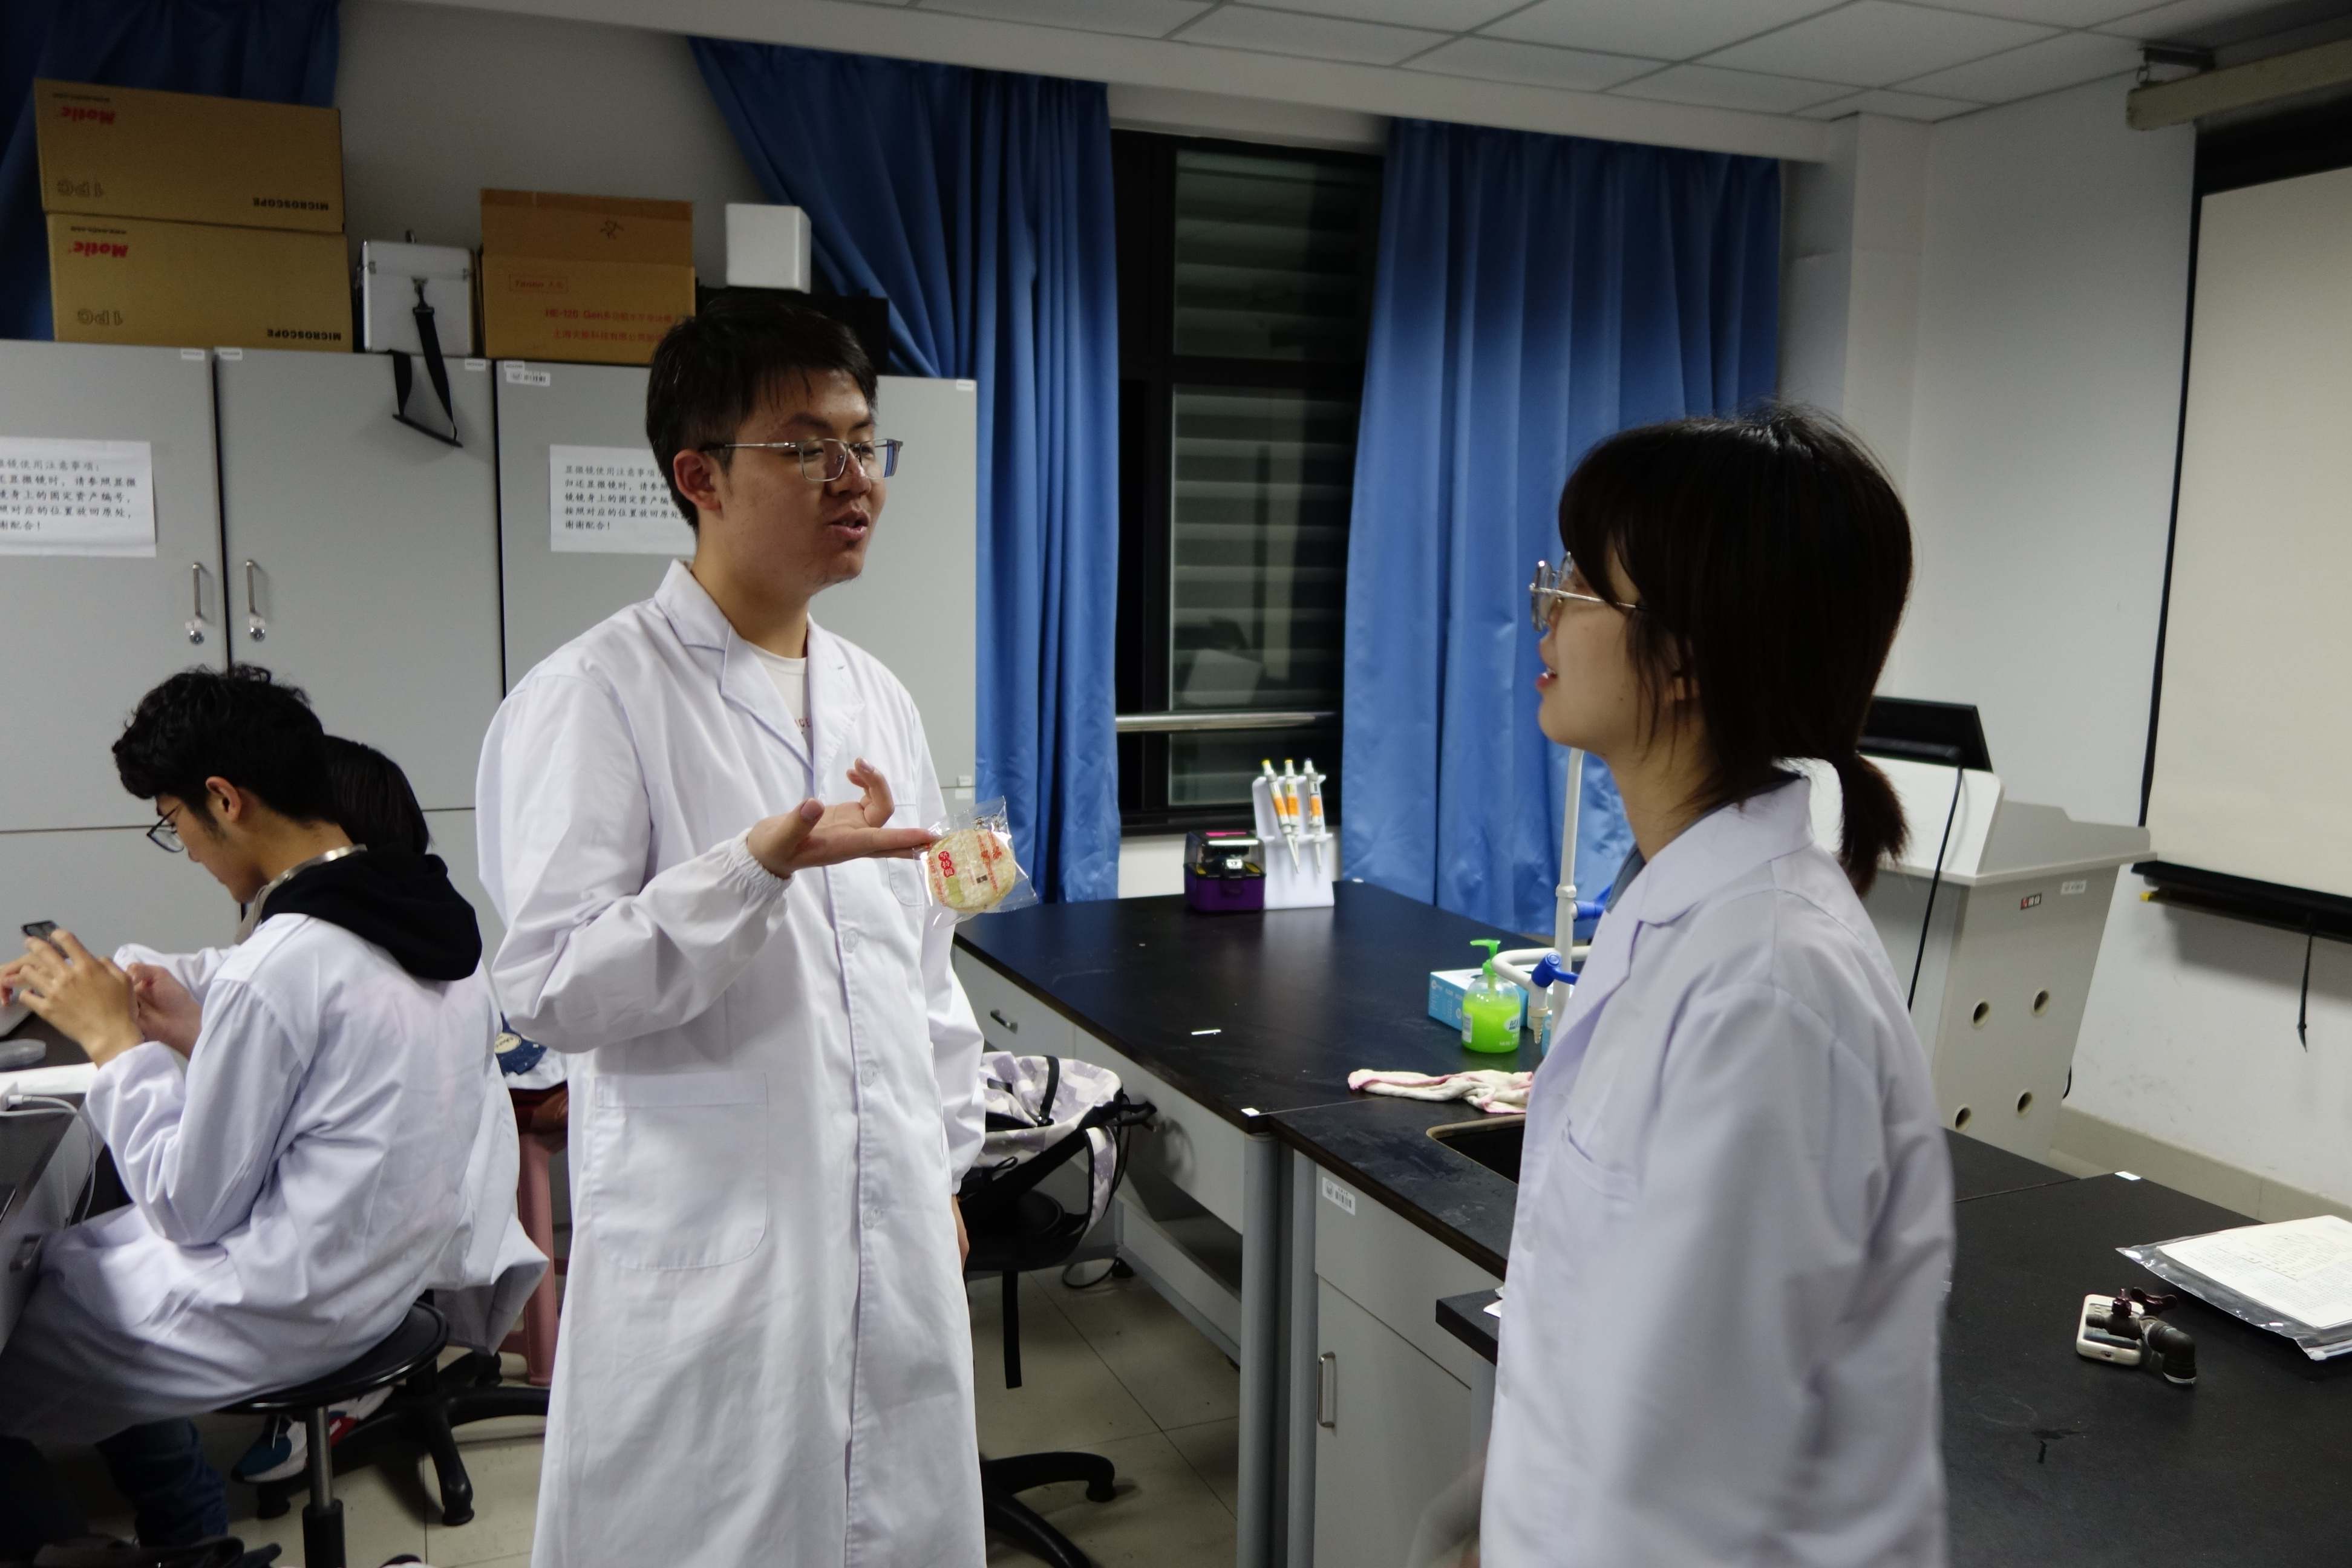
\includegraphics[width=1\textwidth]{image/DSC08163.JPG}
    \caption{From “511”, Micro-bio Lab, 2020\\班干部收缴同学偷偷带入实验室的食品}
    \label{F-01}
\end{figure}
 
该图片拍摄于生物医学教学中心五楼(原道路交通馆),微生物学实验室。按规定,实验室内禁止带入任何食品或饮品。负责的班干部发现一位女同学准备在实验间隙偷吃带入的饼干,故上前收缴制止。

笔者抓拍使用的是索尼小黑卡二代,在室内低光照的环境下快门速度为1/30 秒,光圈f/1.8,焦距10.4 毫米,ISO320。故而视野较宽,在靠近被摄人员的地方也能拍出合适视野的照片。
 
\section{书架一角}
 
\begin{figure}[H]
    \centering
    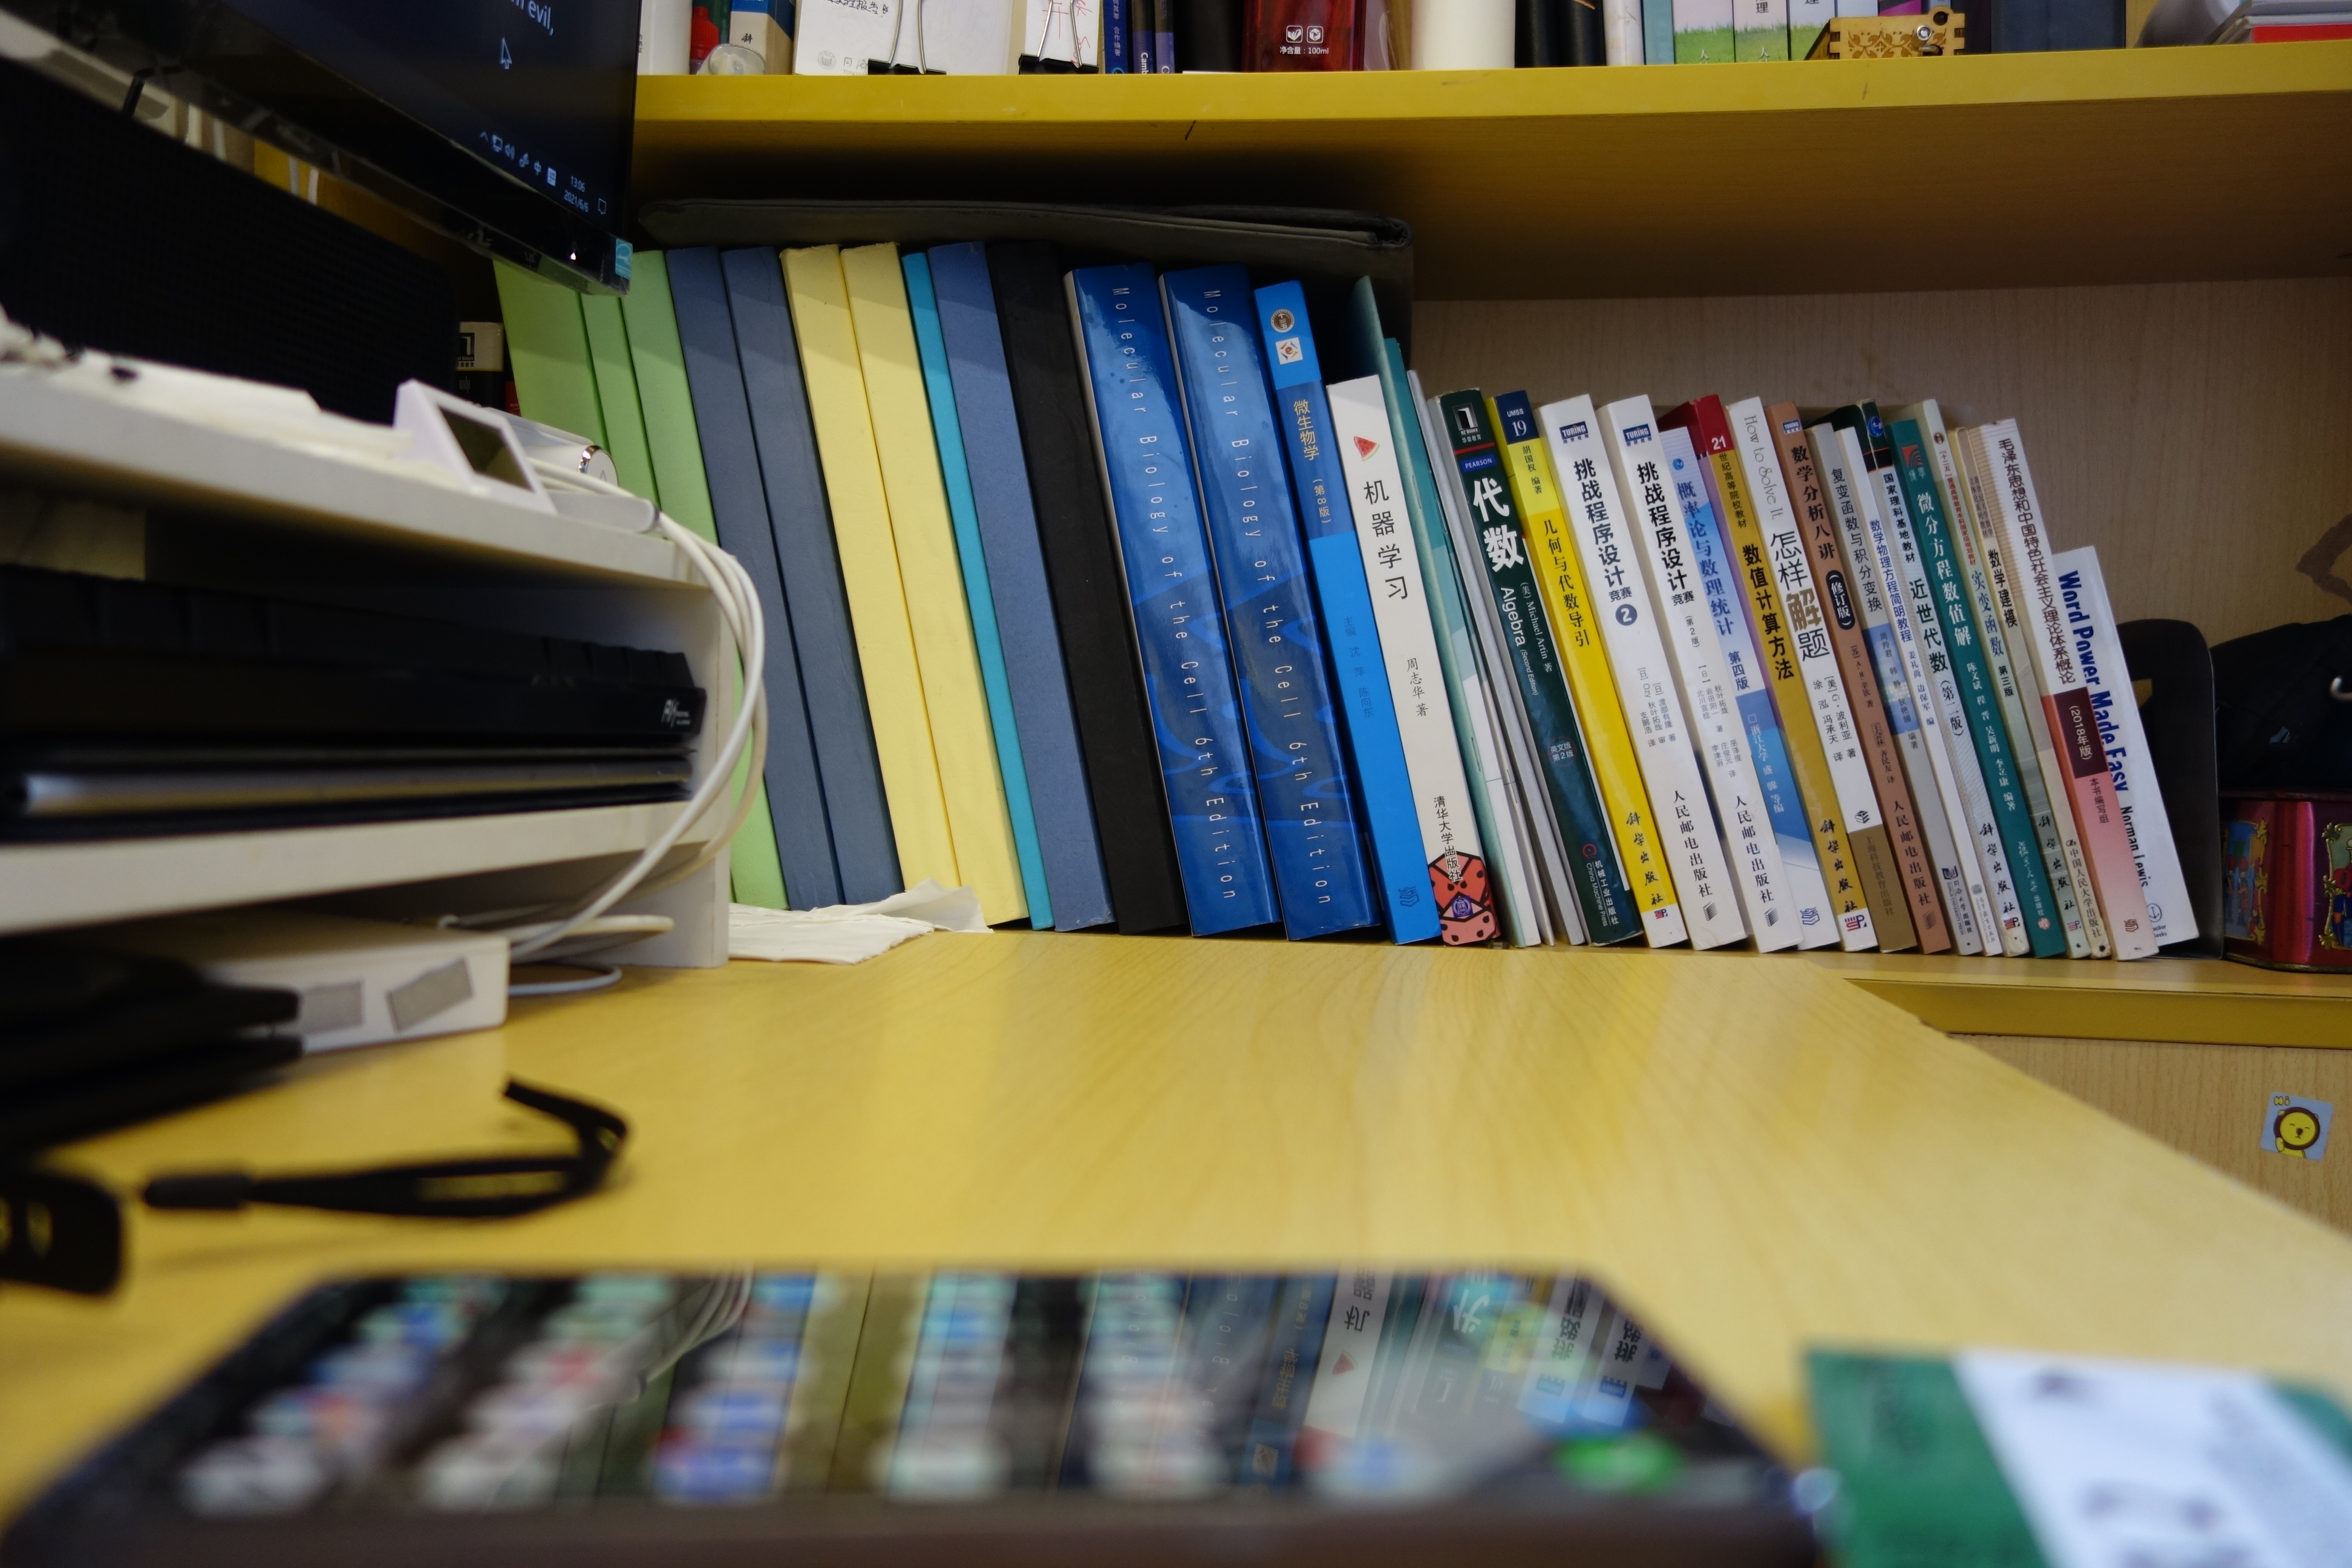
\includegraphics[width=1\textwidth,angle=0]{image/DSC08230.JPG}
    \caption{From “SE10-A205”,2020,  \\ 一些书}
    \label{F-02}
\end{figure}

笔者自己的书架,最下层是最靠手边的部分,放置最常用的书本和讲义。为了使照片不至于单调,笔者适当添加了前景,即对焦没对上的手机和校园卡。

笔者拍摄时使用的是索尼小黑卡二代,在室内低光照的环境下快门速度为1/30 秒,光圈f/1.8,焦距10.4 毫米,ISO250。焦距极短的原因除了黑卡本身的尺寸限制外,还考虑到相机与被摄物体的距离较短,最短对焦范围受限。

%\bibstyle{unsrt}
%\bibliography{references}{}
\end{document}